\documentclass[13pt, t]{beamer}
% Presento style file
\usepackage{config/presento}

% custom command and packages
% custom packages
\usepackage{textpos}
\setlength{\TPHorizModule}{1cm}
\setlength{\TPVertModule}{1cm}

\newcommand\crule[1][black]{\textcolor{#1}{\rule{2cm}{2cm}}}



\title{\Large \hspace{-0.5cm} The speakers of minority languages  \textbf{are more multilingual}}
\author[shortname]{Nina Dobrushina and George Moroz\bigskip}
\institute[shortinst]{Linguistic Convergence Laboratory, NRU HSE, Moscow, Russia}
\date{\begin{center} 16 April 2019 \bigskip \\ {{\color{colorblue} \href{https://ilcl.hse.ru/smallscale/}{\large Typology of small-scale multilingualism} \\ Laboratoire Dynamique du Langage, Lyon, France }\\ \vfill Presentation is availible here: \href{tinyurl.com/y6jjp38y}{\large \color{colorblue}  \textbf{tinyurl.com/y6jjp38y} \hfill 
\includegraphics[height = 2.5cm]{images/01_qrcode}}} \end{center}}

\begin{document}

\begin{frame}[plain]
\maketitle
\end{frame}

\begin{frame}{Multilingualism in Daghestan}
The republic of Daghestan is an area of high language density and diversity. 
\begin{itemize}
\item three language families (the estimated number of languages ranges from 30 to 45):
\begin{itemize}
\item  East Caucasian (Nakh-Daghestanian), 
\item Turkic: Kumyk, Nogai, Azerbaijani
\item Indo-European: Tat and Russian \pause
\end{itemize}
\item The vast majority of Daghestanians are muslims \pause
\item The main occupation in highland villages was shepherding, and, to a certain extent,
crop farming
\item In poor highland settlements people often practiced seasonal jobs outside the village\pause
\item \textbf{Endogamy}: in most Daghestanian villages, partners were taken exclusively from the same family (tukhum) \pause
\item \textbf{Russian} became nowaday a lingua franca, but historically there were several other lingua francas: \textbf{Avar}, \textbf{Azeri}, \textbf{Kumyk}
\end{itemize}
\end{frame}

\begin{frame}{Multilingualism in Daghestan}
\begin{itemize}
\item More than forty languages spoken in Daghestan
\item Many multilingual people
\item Multilingual repertoire is village-based:
\begin{itemize}
\item each village has its own set of second languages
\item incidental knowledge of some language is rare
\end{itemize}
\item Multilingualism is distributed unevenly across villages – some are very
multilingual, some are rather monolingual
\end{itemize}
\end{frame}

\begin{frame}{Problem setting}
\alert{Question:\\}
What influences the richness of language repertoire?\\
\vfill
\alert{Hypothesis:\\}
The number of speakers plays a role\\
(``Numbers count: a larger culture is likely to be a dominant
culture''\\
– Thomason 2001: 6)\\
\vfill
\alert{The aim\\}
To test quantitatively whether the size of language group influences the number of languages it speaks
\end{frame}

\begin{frame}{Our data}
Data obtained during interviews on language usage from about 15 fieldtrips (see \citep{dobrushina2013} for methodology details) and  collected into \textbf{Atlas of Multilingualism in Daghestan} \citep{multidagestan17}:
\begin{itemize}
\item field trips to 17 clusters of villages (2 to 4 villages per cluster); \\ totality of 54 villages
\item 24 langugages (Russian excluded) \pause
\item 3210 people born between 1900 and 1959
\begin{itemize}
\item 1564  females (48.7\%)
\item 1646 males (51.3\%)
\end{itemize}
\item variable containing number of second languages spoken in the village\pause
\item we grouped all languages into three categories according to the number of speakers at the present time
\begin{itemize}
\item {\Large \color{colorbig} \textbf{big}} --- 100 000 speakers and more
\item {\Large \color{colormedium} \textbf{medium}} --- 10 000--30 000 speakers
\item {\Large \color{colorsmall} \textbf{small}} --- one village languages, 1 000--2 000 speakers
\end{itemize}
\end{itemize}
\end{frame}

\begin{frame}{Retrospective family interviews, \citep{dobrushina2013}}
\begin{itemize}
\item Rate of bilingualism at the community level is taken to be a proxy for the intensity of language contact 
\item Short interviews about language repertoire of locals are taken
\item The respondent reports the data not only about himself but also about all his elder relatives whom ((s)he thinks) (s)he remembers
\end{itemize}
\small
\vspace{1mm}
\begin{tabular}{|l|l|}
\hline
Name                                     & Akaj                                      \\ \hline
Born in                                  & Chabanmakhi                               \\ \hline
The interviewer was talking to           & Umaidat                                   \\ \hline
Family relation to the respondent        & Father of Umaidat                         \\ \hline
Years of birth and death                 & 1900 - 1973                               \\ \hline
Native language                          & Kadar Dargwa                              \\ \hline
Education and living outside the village & worked as a mason, also in other villages \\ \hline
Did he read the Koran?                   & Yes, could not translate                  \\ \hline
Did he speak Avar?                       & yes                                       \\ \hline
Did he speak Kumyk?                      & yes                                       \\ \hline
Did he speak Russian?                    & yes                                       \\ \hline
Did he speak any other languages?        & no                                        \\ \hline
Literate in                              & Arabic, Cyrillic                         \\ \hline
\end{tabular}
\end{frame}

\begin{frame}{Why retrospective?}
\begin{itemize}
\item From the establishment of Soviet schools in the 1930s,  Russian quickly spread over Daghestan as L2
\item Traditional patterns of language contact have been almost completely substituted by Russian as a lingua franca
\end{itemize}
\end{frame}


\framepic{images/03_map_930_700}

\framepic{images/04_map_class_930_700}

\framepic{images/05_map_1900_930_700}{\vspace{-2mm}Median number of known L2, people born in 1900--1909}

\framepic{images/06_map_1910_930_700}{\vspace{-2mm}Median number of known L2, people born in 1910--1919}

\framepic{images/07_map_1920_930_700}{\vspace{-2mm}Median number of known L2, people born in 1920--1929}

\framepic{images/08_map_1930_930_700}{\vspace{-2mm}Median number of known L2, people born in 1930--1939}

\framepic{images/09_map_1940_930_700}{\vspace{-2mm}Median number of known L2, people born in 1940--1949}

\framepic{images/10_map_1950_930_700}{\vspace{-2mm}Median number of known L2, people born in 1950--1959}

\framepic{images/11_panel_1100_750}

\begin{frame}{What’s going on in Chuni?}
\begin{itemize}
\item Chuni is Avar village
\item Avar is the biggest Nakh-Daghestanian language (about 700 000)
\item Other Avar villages in our sample are rather monolingual (Chittab, Durangi, Kizhani, Obokh)
\item Chuni is an Avar enclave surrounded by Dargwa varieties (Akusha Dargwa and Tsudakhar Dargwa)
\item Being a linguistic minority, Chuni people speak both languages
\end{itemize}
\end{frame}

\framepic{images/17_Chuni.png}

\begin{frame}{Number of L2 in each village by decade and language category}
\hspace{-0.9cm}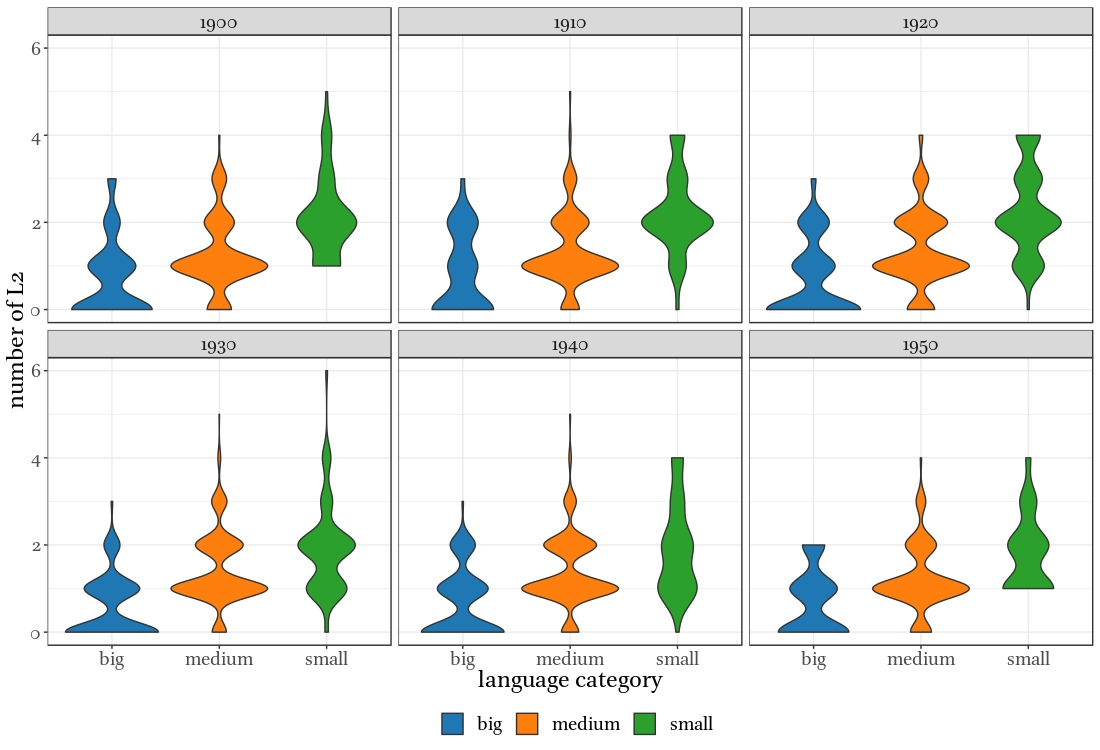
\includegraphics[width=1.08\linewidth]{images/12_panel_1100_750}
\end{frame}

\begin{frame}{Poisson Mixed Effects Model}
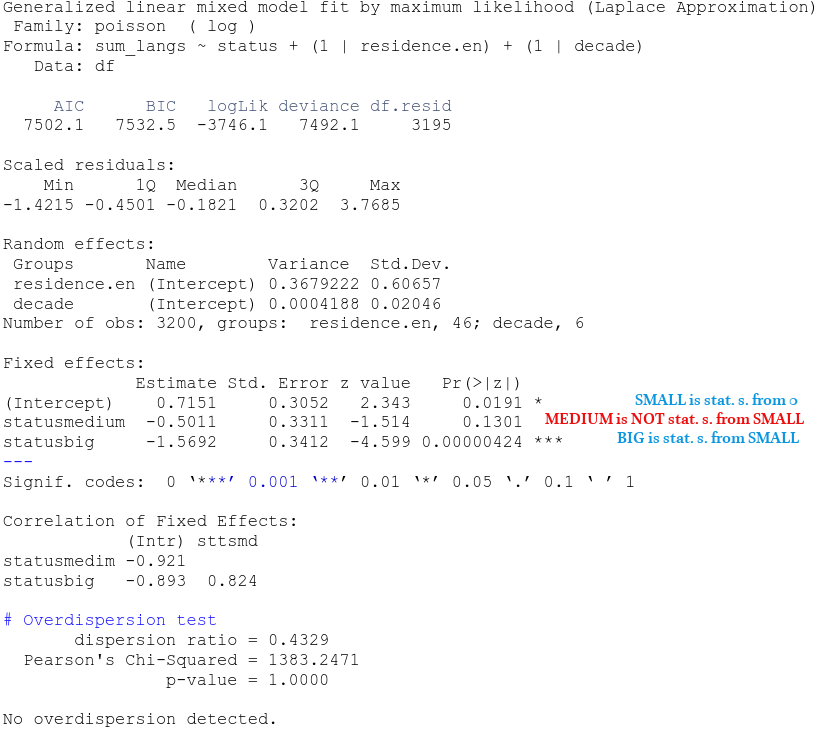
\includegraphics[width=0.87\linewidth]{images/13_poisson}
\end{frame}

\begin{frame}{Poisson Mixed Effects Model: Residuals}
\begin{center}
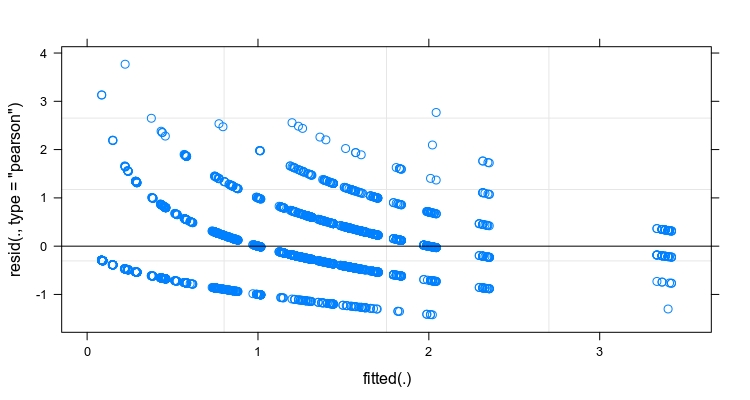
\includegraphics[width=0.75\linewidth]{images/14_poisson_residuals_750_400}\\
\end{center}\pause
Statistical model is not ideal\dots Compare with some examples of ``good'' plots:\\
{\tiny from \url{http://docs.statwing.com/interpreting-residual-plots-to-improve-your-regression/}}
\begin{center}
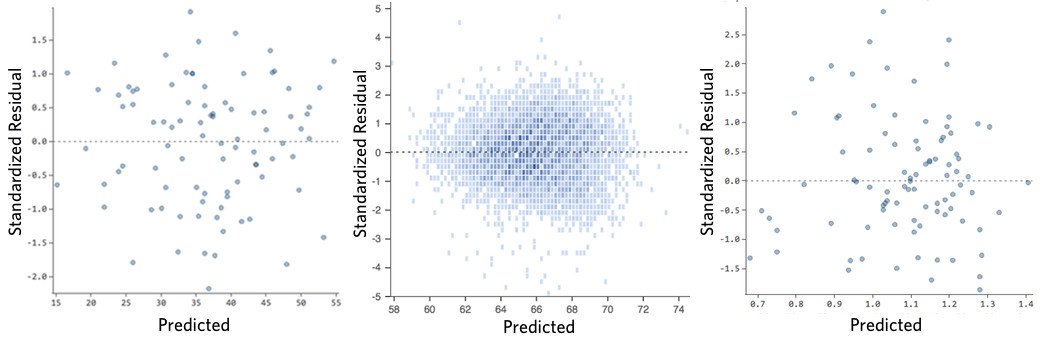
\includegraphics[width=0.7\linewidth]{images/16_good_residuals}
\end{center}
\end{frame}

\begin{frame}{Conclusions:}
\begin{itemize}
\item The variable language size is statistically signifficant.
\item Obtained coefficients could be interpret as following:\\
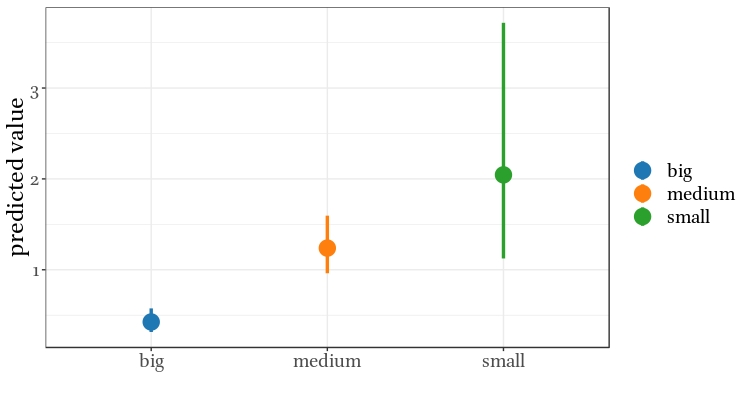
\includegraphics[width=\linewidth]{images/15_predicted_750_400} \pause
\item Special case: Chuni \pause
\item It is not the only case of Daghestanian languages:
\begin{itemize}
\item Circassians in Arabic comunities in Israel \citep{kreindler95}
\item Abaza in Circassian comunities in Russia (personal observations)
\end{itemize}
\end{itemize}
\end{frame}

\framecard[colorblue]{{\color{colorwhite} \Large Send us a letter!\\
nina.dobrushina@gmail.com\\
agricolamz@gmail.com\\ 
\vfill Presentation is availible here: \href{tinyurl.com/y6jjp38y}{\textbf{tinyurl.com/y6jjp38y}}\\
\vfill  
\includegraphics[height = 3cm]{images/02_qrcode}}\\
\vfill {\small  \color{colorwhite} All visualisation and statistical analysis were made in \texttt{R}~version~3.5.3~\citep{r19} with packages \texttt{ggplot2}~\citep{wickham16}, \texttt{lme4}~\citep{bates15}, \texttt{lingtypology}~\citep{moroz17}}}

%\begin{frame}[allowframebreaks]{Список литературы}
\begin{frame}{References}
\footnotesize
\bibliographystyle{config/chicago}
\bibliography{bibliography}
\end{frame}

\end{document}